\documentclass[../dissertation.tex]{subfiles}

\begin{document}

\chapter{TD-Learning and Deep Reinforcement Learning for Importance Sampling Light Paths}
\label{chap:td_deep_sampling}

Monte Carlo Integration, importance sampling, Monte Carlo path tracing, reinforcement learning and the link between temporal difference learning and light transport have all been introduced. So now it is finally time to combine all of these concepts to build path tracing algorithms for Importance sampling. 

In this section I introduce two path tracers I have implemented to assess their ability in reducing image noise in Monte Carlo path tracing with a fixed number of sampled light paths per pixel. The first is based on a method introduced by Nvidia \cite{dahm2017learning} which I refer to as the Expected Sarsa path tracer. The other I refer to as the Neural-Q path tracer which I have designed. Both of which progressively reduce the number of zero-contribution light paths sampled during rendering, reducing the variance in the Monte Carlo approximation of a pixels colour. Ultimately, reducing the noise in rendered images. 

\section{The expected Sarsa Path Tracer}
\label{sec:expecte_sarsa_path_tracer}

The Expected Sarsa path tracer was first introduced by Nvidia \cite{dahm2017learning} to apply the derived  Expected Sarsa learning rule for learning the incident radiance in a given direction on a position, which was derived in Equation \ref{eq:mc_expected_sarsa_td_learning}:

$$Q(x, \omega) \leftarrow (1 - \alpha) \cdot Q(x, \omega) + \alpha \cdot \left( L_e(y, -\omega) +\frac{2 \pi}{n} \sum_{k=1}^{n-1} Q(y, \omega_k) f_s(\omega_k, y, -\omega) \cos(\theta_k)  \right)$$

I will now introduce my implementation of the algorithm which uses it to progressively reduce the number of zero-contribution light paths sampled in a path tracer, which can reduce noise in rendered images significantly. 

\subsection{The Irradiance Volume}
The derived Expected Sarsa learning rule requires some sort of data-structure for looking up and updating the incident radiance on a point $x$ from direction $\omega$, which from here on I will refer to as a Q-value. Therefore, the main requirement of the data structure is that it has some way of representing a discrete set of angles ($\omega_k$) in a hemisphere located at a position $x$ and oriented to the surface normal at $x$. The Irradiance Volume data structure \cite{greger1998irradiance} meets this requirement.\\

\begin{figure}[h]
\begin{center}
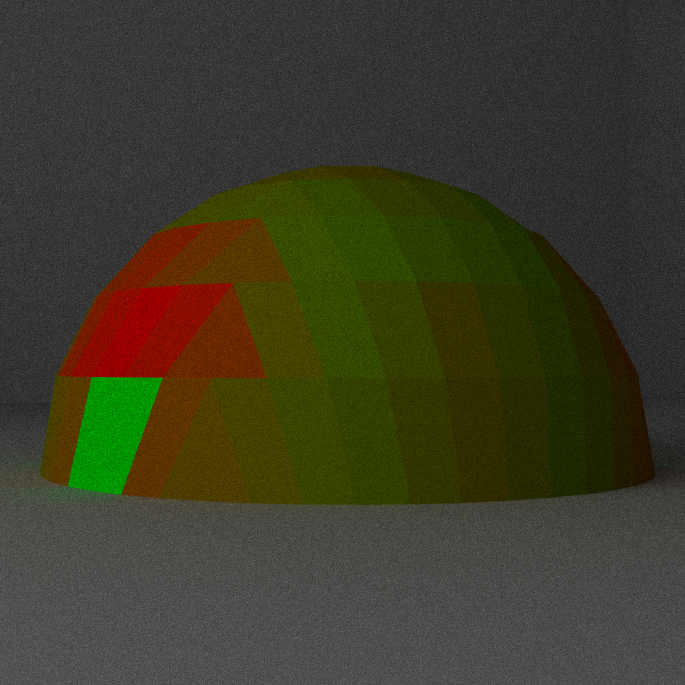
\includegraphics[width=0.3\textwidth]{images/renders/hemispheres/irradiance_volume.png}    
\end{center}
\caption{An Irradiance Volume. Each sector holds the incoming radiance $L_i(x,\omega_k)$, the more green a sector is the lower the stored radiance in that sector, the more red a sector is the higher the stored radiance in that sector. }
\label{fig:irradiance_volume}
\end{figure}

Originally designed to be used for pre-computation of radiance values which are looked up at runtime to approximate global illumination, the Irradiance Volume data structure is essentially a discretized version of a hemisphere which is visually represented in Figure \ref{fig:irradiance_volume}. The image shows the discrete sectors which make up a hemisphere, this was implemented by converting a 2D square grid into the 3D hemisphere shown, which is known as an adaptive quadrature. Where all sectors in the 2D grid have an equal area and a mapping introduced in \cite{shirley1994notes} converts the 2D grid coordinates into a hemisphere made up of sectors in 3D space. The mapping ensures the hemisphere sectors remain equal to one another, meaning the discrete set of direction represented by the hemisphere are of equal angles apart from one another.\\

\begin{figure}[!htb]
\centering
\minipage{0.32\textwidth}
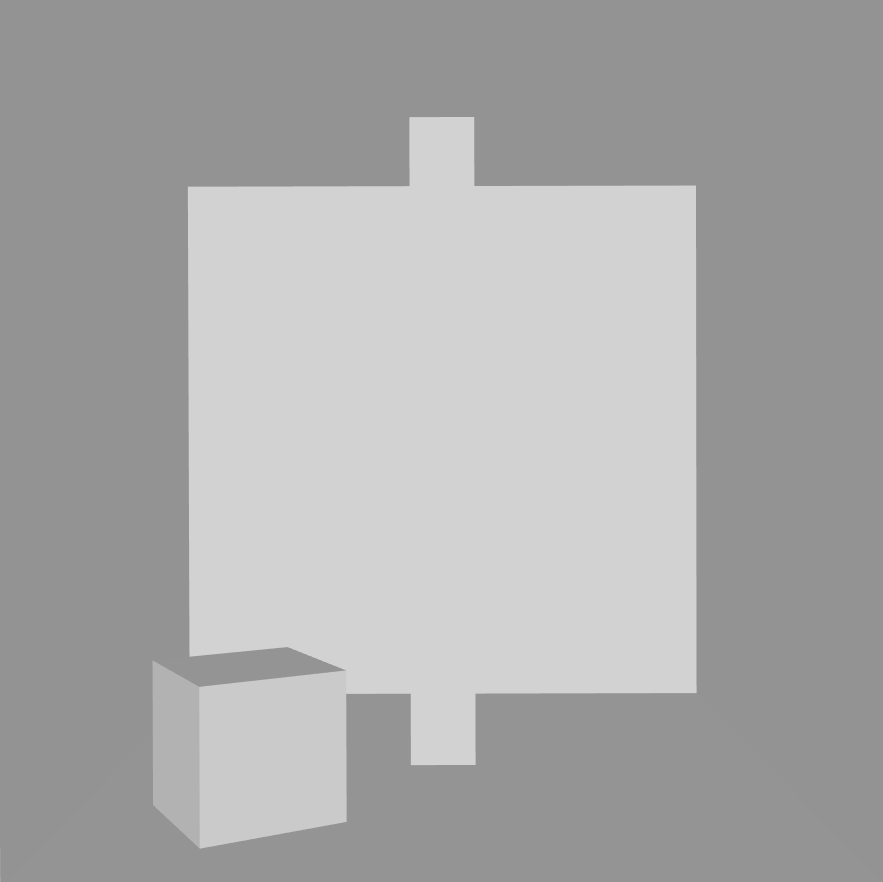
\includegraphics[width=1\textwidth]{images/renders/simple_room/geometry.png}
  \subcaption{Representation of the scenes geometry meshes}
\endminipage\hfill
\minipage{0.32\textwidth}
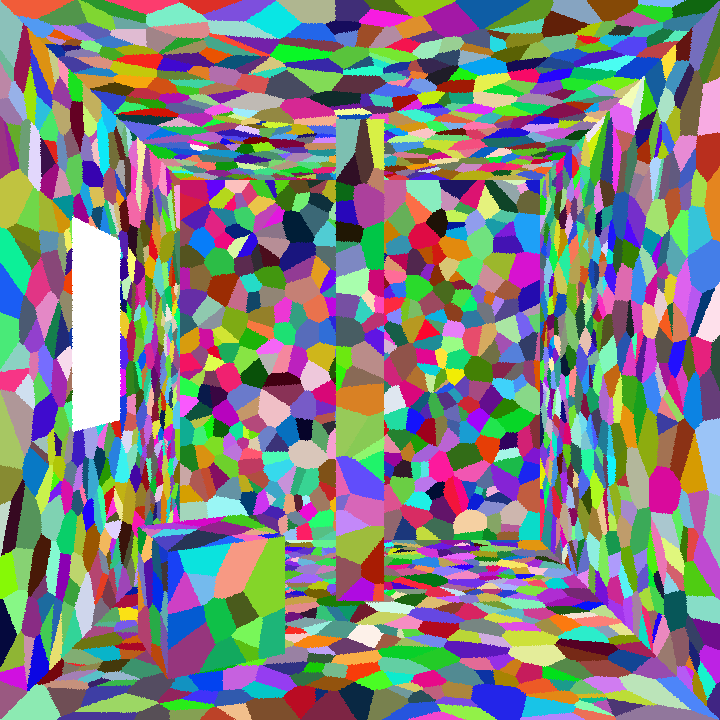
\includegraphics[width=1\textwidth]{images/renders/simple_room/voronoi.png}
   \subcaption{Voronoi Plot of Irradiance Volume locations}
\endminipage\hfill
\minipage{0.32\textwidth}
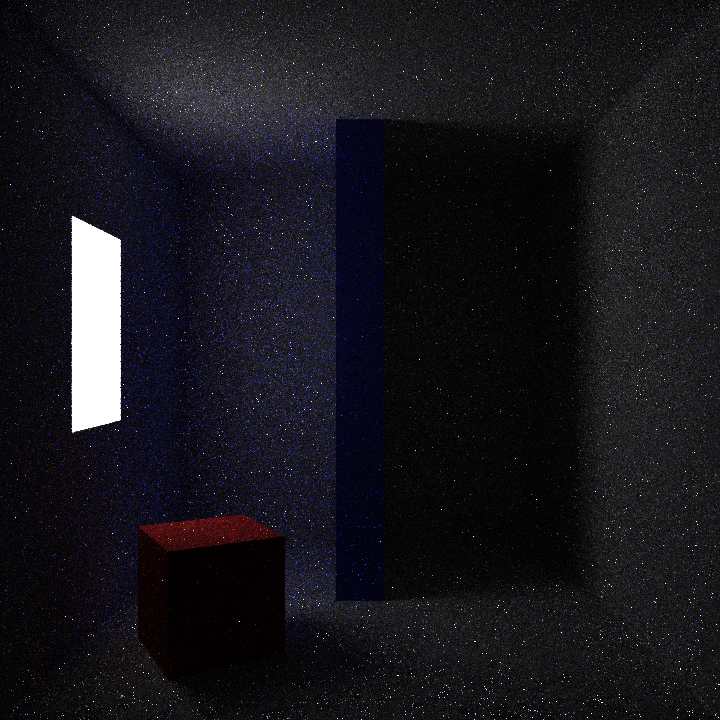
\includegraphics[width=1\textwidth]{images/renders/simple_room/reinforcement_16.png}
  \subcaption{Expected Sarsa path tracer with 16 SPP}
\endminipage
\caption{An example of discretizing location in the scene into Irradiance Volume locations. The geometry mesh (a) is used to uniformly sample Irradiance volume positions. Image (b) shows a voronoi plot for the Irradiance Volumes in the scene, where each pixel is coloured to the represent its closest Irradiance Volume, so each sector of colour in (b) represents a different Irradiance Volume location. Finally (c) gives a render using the Expected Sarsa path tracer based on Algorithm \ref{alg:expected_sarsa_pathtracer}.}
\label{fig:scene_discretization_example}
\end{figure}

Each sector of the Irradiance Volume is then used to store the current approximation of incident radiance in the incident direction formed by the unit vector from centre of the sector to $x$. Therefore, an Irradiance Volume stores the incident radiance (Q-value) for a given position $x$ (state) from each direction $\omega_k$ (action), for all sectors $\forall k = 1,...,n$ in the hemisphere located at $x$. In order to store Q-values across the scene, Irradiance Volumes can be uniformly sampled over the scenes geometry as shown in Figure \ref{fig:scene_discretization_example}. Then to lookup a radiance/Q-value for a given position $x$ in direction $\omega_k$, a nearest neighbour search is performed to find the closest Irradiance volume to position $x$, then retrieve the Q-value from the sector at index $k$. Giving a lookup and update time of $O(\log n) + O(1) = O(\log n)$ when using the KD-Tree data structure for nearest neighbour search \cite{bentley1975multidimensional}.  Lookup and update procedures from the Irradiance volumes in the scene is all that is needed to apply the Expected Sarsa learning rule in Equation \ref{eq:mc_expected_sarsa_td_learning}. The entire collection of Irradiance Volumes in a scene can be thought of as a large 5D table ($x \in \mathbb{R}^3, \omega \in \mathbb{R}^2$) to store the current incident radiance approximation at each point. Expected Sarsa and all other TD-learning methods presented in section \ref{sec:td_learning} are know as tabular methods, and I will refer to the table described as the Q-table for the scene.\\

%TODO Explain KD-Tree?

At each Irradiance Volume the radiance distribution is stored. The radiance distribution for each radiance volumes is a probability distribution over the $n$ Q-values (incoming radiance estimates) stored by the radiance volume. As described in section \ref{sec:td_light_transport}, a direction to continue a light path in can be sampled proportionally to the radiance distribution of the closest radiance volume to the a light paths intersection point. This distribution is also used as the probability density function in the Monte Carlo path tracing colour estimate for a pixel (Equation \ref{eq:rendering_eq_monte_carlo}). Due to this, as the radiance estimate held in each of the $n$ sectors of every radiance volume improves with the number of rendered frames, the radiance distribution will come closer a normalized version of the true function describing the incoming radiance on point $x$. Therefore, the variance in the colour estimate for a light path through a given pixel will reduce for the same number of samples used, progressively reducing image noise.

\subsection{Expected Sarsa Path Tracing}
\label{sec:expected_sarsa_path_tracer}

The Expected Sarsa based path tracing algorithm is very similar to the original forward path tracer introduced in Algorithm \ref{alg:forward_path_tracing}. The algorithm learns online, meaning after every rendered frame pixel values are likely to have a lower variance due to a reduction in the number of zero contribution light paths sampled. Initially, radiance volumes are sampled uniformly across the room with all Q-values initialised to a small constant proportional to the number of sectors on each hemisphere $k$. This encodes the assumption that initially the radiance in all directions from any given point in the room is equal, as initially there is no prior knowledge of any radiance values $Q(x, \omega)$. With the radiance volumes set up, every frame $N$ sampled light paths are traced through each pixel from the camera and into the scene to find its average colour estimate using Algorithm \ref{alg:expected_sarsa_pathtracer}. Algorithm \ref{alg:expected_sarsa_pathtracer} updates the radiance distribution stored in by each Irradiance Volume after every rendered frame using the updated $Q(x, \omega_k)$ values stored. Meaning the next frame will importance sample from the new updated radiance distribution estimate held by every Irradiance Volume. The three additions to this algorithm from the forward path tracer in Algorithm \ref{alg:forward_path_tracing}, are as follows:

\subsubsection*{Addition 1: Sample directions proportional to closest radiance distribution}
The direction to continue the light path in is sampled proportional to the Q-values stored in the closest Irradiance Volume to position $y$ by using the stored radiance distribution in the closest Irradiance Volume.  Inverse transform sampling \cite{devroye2006nonuniform} is used to sample a direction from the stored radiance distribution. Inverse transform sampling is where a random number $r \in [0,1]$ is sampled, then the largest number $x$ from the domain of the cumulative distribution $P(X)$ is returned where $ P(-\infty < X < x) \leq r$. 

\subsubsection*{Addition 2: Update stored Q-values}
Once the ray has intersected with a position in the scene $y$ from a position $x$, update the radiance estimate $Q(x, \omega)$ using the Expected Sarsa learning rule derived in Equation \ref{eq:mc_expected_sarsa_td_learning}. This is based on the radiance emitted from $y$ in direction $-\omega$ and the outgoing radiance estimate in direction $-\omega$ from point $y$ described by the summation. The summation involves summing all Q-values for the closest radiance volume to position $y$. Each of which are multiplied by BRDF of the surface at $y$, as well as the cosine of the angle between the sector direction for the Q-value ($\omega_k$) and the surface normal $y$.

\subsubsection*{Addition 3: Update Irradiance Volume Distributions}
Update every radiance volumes radiance distribution in the scene by normalizing the radiance volumes updated $Q(x, \omega_k)$ values. 



\begin{algorithm}[H]
\label{alg:expected_sarsa_pathtracer}
\SetKwProg{Fn}{Function}{ }{end}
\SetAlgoLined
 \Fn{renderImage(camera, scene)}{  
   \For{$i = 1$ \KwTo $N$}{
     \For{$p$ \In $camera.screen$}{
         $ray \leftarrow \text{initializeRay}(p, camera)$\\
         \For{$j=1$ \KwTo $\infty$}{
         $(y, \mathbf{n}, L_e) \leftarrow \text{closestIntersection}(ray, scene)$\\
         \If{$j > 1$}{
            \tcc{Addition (1)}
            $(\omega_i, \rho_i, f_s) \leftarrow \text{sampleRayDirFromClosestRadianceDistribution}(y)$\\
            \tcc{Addition (2)}
            $Q(ray.x, ray.\omega) \leftarrow (1 - \alpha(ray.x, ray.\omega)) \cdot Q(ray.x, ray.\omega) + \alpha(ray.x, ray.\omega) \cdot \left( L_e +\frac{2 \pi}{n} \sum_{k=1}^{n-1} Q(y, \omega_k) f_s(\omega_k, y, -ray.\omega) \cdot (\omega_k \cdot \mathbf{n})  \right)$\\
         }
         \If{$\text{noIntersection}(y) \ \Or \ \text{areaLightIntersection}(y)$}{
             $ray.throughput \leftarrow ray.throughput \cdot L_e$\\
             $\text{updatePixelColourEstimate}(p, ray.throughput)$\\
             $\Break$
          }
          $ray.throughput \leftarrow ray.throughtput \cdot f_s \cdot (\omega_i \cdot \mathbf{n}) / \rho_i$\\
          $ray \leftarrow (y, \omega_i)$
       }
   }
  }
  \tcc{Addition (3)}
  $\text{updateIrradianceVolumeDistributions()}$
 }
 \caption{Expected Sarsa path tracer pseudo code following Nvidia's method in \cite{dahm2017learning}. Given a camera position, scene geometry, this algorithm will render a single image using a tabular Expected Sarsa approach to progressively reduce image noise. Where $N$ is the pre-specified number of sampled light paths per pixel.}
\end{algorithm}

\subsubsection*{Monte Carlo Integration}

Due to the importance sampling from addition (2), the probability density function over all possible sampled directions $\Omega$ at location $x$ is no longer uniform. Instead it is equal to the normalized Q-values for the closest Irradiance Volume to the point $x$, which is the stored radiance distribution. Therefore the evaluated probability density function $\rho_i$ at intersection point $x$, at incident direction $\omega_i$ must also be evaluated using the radiance distribution to correctly apply Monte Carlo Integration. To do so I have derived an Equation \ref{eq:mc_expected_sarsa_pdf} to determine the value $\rho_i$.

\begin{equation}
\label{eq:mc_expected_sarsa_pdf}
\rho_i = Q_p(x, \omega_k) \cdot n \cdot \frac{1}{2 \pi} = \frac{Q_p(x, \omega_k) \cdot n}{2 \pi}
\end{equation}

\noindent
Where:
\begin{conditions}
 Q_p(x, \omega_k)   & Normalized Q-value from the Irradiance Volume closest to $x$ at sector $k$\\
 n   & Total number of sectors in an Irradiance Volume \\
\end{conditions}

The reasoning behind this value $\rho_i$ is that $\frac{1}{2\pi}$ represents the probability density function ($pdf$) evaluated at any point when directions are randomly sampled in the hemisphere $\Omega$. However, the Irradiance Volume splits the hemisphere into discrete sectors, but each sector represents a continuous set of angles. Therefore if the probability of sampling a ray in each sector were constant $c$, $Q_p(x,\omega_k) = c$ $\forall k < n$, the $pdf$ would remain constant:

$$ \frac{Q_p(x, \omega_k) * n}{2\pi} = \frac{1}{2\pi}$$

However, the approximated radiance may vary across sectors, causing the associated $pdf$ to vary across sector due to $Q_p(x, \omega_k)$. This was not the case previously prior to importance sampling, where direction were sampled randomly over a unit hemisphere making a the $pdf$ is uniform. The diagram in Figure \ref{fig:pdfs} highlights these differences.

\begin{figure}[h]
\centering
\minipage{0.32\textwidth}
  
\includegraphics[width=\textwidth]{images/uniform_pdf.png}   
  \subcaption{Hemisphere with a uniform $pdf$}\label{fig:uniform_pdf}
\endminipage\hspace{5em}
\minipage{0.32\textwidth}
  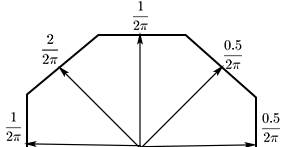
\includegraphics[width=\textwidth]{images/not_uniform_pdf.png}
  \subcaption{Irradiance Volume with a non-uniform $pdf$}\label{fig:not_uniform_pdf}
\endminipage
\caption{A 2 dimension view of a subset of values from two probability density functions ($pdf$). One for a unit hemisphere (left) with a uniform $pdf$. One for an Irradiance Volume (right) with non-uniform pdf. Where the arrows represent sampled directions and the values at the end are the evaluated $pdf$ values for each direction.}
\label{fig:pdfs}
\end{figure}

\subsubsection*{Consistency}
It is important for the modified path tracing algorithm to converge to ensure consistency, meaning all introduced artefacts such as image noise are guarenteed to vanish over time \cite{dahm2017learning}. A decaying learning rate for $\alpha$ can be used to do so, see Equation \ref{eq:decay_lr}. Where $\text{i}(rv, \omega_k)$ is the number of times the rendering algorithm has updated the Q-value of the Irradiance Volume $i$ for sector $k$ representing angle $\omega_k$.

\begin{equation}
\label{eq:decay_lr}
\alpha(x, \omega) = \frac{1}{1 + \text{visits}(x, \omega_k)}
\end{equation}

Now, while $Q(x, \omega_k)$ does converge, it does not necessarily converge on the true radiance $q_*(x, \omega_k)$. This is due to the discretization of the action/direction into sectors which make up a hemisphere. If the number of sectors was infinite then the algorithm would converge on the true radiance by the law of large number applied to Equation \ref{eq:mc_expected_sarsa_td_learning}. Clearly this is not possible, but later I discuss how increasing the number of  sectors on the Irradiance Volume affects the number of zero-contribution light paths. Another issue is Q-values will not be visited the same number of times during rendering. For example Irradiance Volumes located in places which are in the cameras view will be visited far more, so images rendered of the scene which have been in the cameras view for the longest are likely to have the lowest variance in pixel colours. This is a problem, as parts of the scene may look particularly noisy compared to others as the camera begins to move round the scene.

\pagebreak

% -----------------------------------------------------------------------------

\section{The Neural-Q Path Tracer}

Up to now I have only spoke of TD-learning techniques which involve use a tabular approach to approximate the the optimal value function. However, it is possible to instead use a Neural Network as a non-linear function approximater for the optimal value function \cite{deep_rl_function_approx}. Following this I introduce an artificial neural network architecture capable of learning the incident radiance on any point in a scene from a discrete set of angles. I then propose the Neural-Q path tracing algorithm I have designed and implemented which uses the neural networks approximations for importance sampling direction to continue light paths in.

After, I take a slight detour to review the new materials that have been recently published on neural networks for importance sampling in Monte Carlo path tracing. The materials that focus on neural importance sampling for light path construction were published during the execution of the project, so it is important to find out where my Neural Q-learning algorithm sits compared to these new state of the art methods.

\subsection{Introduction to Deep Reinforcement Learning}

\subsubsection{Value Function Approximation}
Observe the optimal value function introduced in section \ref{sec:optimal_value}, Equation \ref{eq:optimal_value}:

$$ q_*(s,a) = \max_\pi q_\pi(s,a)$$

Recall this is simply a function which given a state and action, outputs a scalar representing the value of that state action pair. Therefore, rather then approximating it using a tabular form, instead one can learn the a functions parametrized functional form with a weight vector $\theta = (\theta_0, ..., \theta_n) \text{ where } \theta_i \in \mathbb{R}$. This turns the task of approximating the value function into a function approximation problem, for which there are many possible methodologies. To name some, Coarse coding, Decision Trees, Nearest Neighbour, Fourier basis, and Artificial Neural Networks (ANNs) \cite{sutton2011reinforcement}. Function approximators other than ANNs have been successful for a range of reinforcement learning problems, whilst maintaining both data and computational efficiency \cite{sutton1996generalization, konidaris2011value, uther1998tree}. However, I will be using an ANN for value function approximation due to its capabilities of learning a non-linear functions, and its performance in the presence of a large amount of training data \cite{lecun2015deep}. The exact reasons these benefits are capitalized on will become more apparent later. By using a ANN for function approximation, the technique is now known as Deep Reinforcement Learning.

\subsubsection{Stochastic Gradient Descent}
The goal of the artificial neural network is to learn the value of the function parameters $\theta$ such that the functions loss over all possible state-action pair inputs is minimised. In the case of ANNs the parameters $\theta$ are the weights for the connections between neurons. For stochastic gradient descent a differentiable loss function which takes parameter vector $\theta$ as input and outputs a scalar loss value is required. The method from here on is to move the parameter values $\theta$ in the direction of the negative gradient to minimise the loss function:

$$ \triangle \theta = -\frac{1}{2} \alpha \triangledown_\theta J(\theta)$$

Where $\alpha$ is the step-size parameter. An example loss function for approximating the optimal value function $q_\pi$ is given in Equation \ref{eq:example_loss}. 

\begin{equation}
J(\theta) = \sum_{s \in \mathcal{S}} \sum_{a \in \mathcal{A}} (q_\pi(s,a) - q_\theta(s,a))^2
\label{eq:example_loss}
\end{equation}

\noindent
Where:
\begin{conditions}
J(\theta) & The loss value function for the current parameter values $\theta$\\
q_\pi(s,a) & The value function under policy $\theta$ for the state-action pair\\
q_\theta(s,a) & Current approximation of the value function under policy $\theta$ for the state-action pair 
\end{conditions}

If plenty of data was available for $q_\pi(s,a)$ for many state actions pairs $(s,a)$, it would be possible to train an ANN to approximate the optimal value function $q_\pi$. By simply running a forward pass on the ANN to compute $q_\theta(s,a)$ for a given state-action pair as input, then calculating the loss $J(\theta)$ using the ground truth $q_\pi(s,a)$. Then, by using the backpropagation algorithm to calculate the partial derivatives w.r.t the loss, the parameters values $\theta$ can be updated using an optimizer such as Adam. The issue is $q_\pi$ is unknown and no training data is initially available for the training procedure just described. Instead, deep reinforcement learning uses online training procedures closely resembling the TD-learning methods introduced in section \ref{sec:td_learning} for function approximation.

\subsubsection{Bootstrapping}
\label{sec:bootstrapping}

Following TD-learning, as the optimal value function $q_*$ (or $q_\pi$ in the previous section) is not available, it is possible to instead bootstrap using the current estimate of the value function \cite{deep_rl_function_approx}. Recall that bootstrapping for the value function is when the updated current estimate of the optimal value function for a state-action pair is partially based on new experience data, and the current estimated value of the next selected state-action pair when following policy $\pi$. An example of this is the off-policy method Q-learning presented in section \ref{sec:td_learning}, Equation \ref{eq:q_learning}. Equation \ref{eq:td_error_q_learning} gives what is known as the TD error ($\delta_t$) for Q-learning at time step $t$. It is called an error as it gives the difference between the current estimate $Q(S_t, A_t)$ and the better estimate $R_{t+1} + \gamma \max_a Q(S_{t+1}, a)$. Notice that the TD error is an estimate that has been made at time step $t$, meaning the error depends on the next state and the next reward which can both change across time steps.

\begin{equation}
\delta_t =\left(R_{t+1} + \gamma \max_a Q(S_{t+1}, a)\right) - Q(S_t, A_t)
\label{eq:td_error_q_learning}
\end{equation}

It is this TD error that can be used to form the loss function for an ANN to approximate the value function, as shown in Equation \ref{eq:loss_q_learning}. The gradient of this loss function can be calculated by Equation \ref{eq:q_learning_derv_loss} which is used with an optimizer for updating the parameters $\theta$ during learning. This is the only deep reinforcement learning rule I shall be using from here on for the Neural-Q path tracer.

\begin{equation}
J(\theta) = \left(R_{t+1} + \gamma \left[ \max_a \hat{q_\theta}(S_{t+1}, a) \right] \right) -
\hat{q_\theta}(S_t, A_t)
\label{eq:loss_q_learning}
\end{equation}

\begin{equation}
\triangledown _\theta J(\theta)  = \left( \left(R_{t+1} + \gamma \left[ \max_a \hat{q_\theta}(S_{t+1}, a) \right] \right) -
\hat{q_\theta}(S_t, A_t) \right) \triangledown_\theta \hat{q_\theta}(S_t, A_t)
\label{eq:q_learning_derv_loss}
\end{equation}

\noindent
Where:
\begin{conditions}
\triangledown_\theta & Gradient w.r.t $\theta$\\
\hat{q_\theta} & The current approximation of the value function given by an ANN\\
\left[ . \right] & Stop gradient, meaning the value is taken as just a scalar input during backpropagation
\end{conditions}

Unfortunately due to the use of function approximators for TD-learning methods, the methods are no longer proven to converge on the optimal policy $q_*$. That said, in general these methods perform well in practice for appropriate use cases \cite{lillicrap2015continuous, mnih2013playing}, and generally learn faster than the other option of Monte Carlo Reinforcement Learning with function approximation \cite{sutton2011reinforcement}.

\subsection{Deep Reinforcement Learning Motivation}
\label{sec:deep_rl_motivation}

Like tabular TD-learning methods, I attempt to a deep reinforcement learning method to approximate the incident radiance from a set of discrete directions $\omega_k$ where $k = 0,..., n$ from point $x$ in the scene ($L_o(x, \omega_k)$), where $n$ is the number of discrete directions in the hemisphere. Then, when sampling direction to continue light paths during path tracing, the incident radiance estimate from each discretized direction is normalized, forming a distribution known as the radiance distribution, see section \ref{sec:irradiance_volume}. A good approximation of the radiance distribution at a point can be used in importance sampling directions for light path construction during Monte Carlo path tracing in order to reduce image noise (see section \ref{sec:monte_carlo_path_tracing}).\\

Unlike the Expected Sarsa tabular approach, function approximation has the ability to generalize the value over state-action pairs. In other words, the tabular approach requires a single entry for every possible state-action. So, if an update is made to a state-action pair, it affects that state-action pair value alone. In the case where there are many states (potentially infinitely many) state-action pairs may not be updated often due to the number of them. This means they will be updated infrequently, making learning slow. It may not even be possible to store such a number of state-action pairs. Using an ANN or any function approximator allows one to model a potentially infinite state space and generalize for the valuation of for unseen state-action pairs, which applies well to rendering as the number of unique positions in the scene is infinite. However, this comes at the cost of updating weights in the ANN can affect the valuation of multiple states, making it impossible in practice to predict the optimal value for every state-action pair, unlike the tabular case. This causes proofs for convergence on the optimal value function, $q_*(s,a)$ to break down.\\

Previously, I highlighted that I chose an ANN as the function approximator for the Neural-Q path tracer due to its ability to model non-linear functions well in the presence of a large amount of training data. When approximating the incident radiance $L_i(x, \omega)$ for all possible positions in the scene, the radiance distribution at any point in the scene can be a non-linear function due to the way light paths randomly reflect off complex geometry in a scene. Therefore, learning the radiance distribution for all points in a arbitrary scene requires a non-linear function approximator. In terms of training data, the rendering process samples light paths to approximate radiance which can be used for training. This means as much training data as needed can be generated during the rendering process.\\

The range of improvements to the approximation of incoming radiance that can be potentially made by using ANNs makes it a clear area to investigate. However, this is all conditioned on if it is possible for an ANN to learn the radiance distribution for any point in an arbitrary scene.


\subsection{Deep Q-learning for Light Transport}

In order to use deep reinforcement learning to learn the incident radiance on a point from a given direction in the scene, I must first derive a loss function for which the neural network will be trained with in a similar way done for the Expected Sarsa learning rule in section \ref{sec:td_light_transport}. However, instead of using Expected Sarsa, I find a loss function using the deep Q-learning rule introduced in Equation \ref{eq:loss_q_learning}. This choice was made primarily due to its proven success when used to approximate the optimal value function for a variety of Atari games \cite{mnih2013playing}.

Once again, the rendering equation from section \ref{sec:rendering_equation} states the radiance in an outgoing direction $\omega$ from point $x$ is equivalent to the emitted radiance in the direction plus the reflected radiance in the direction:

\begin{equation}
L_o(x, \omega) = L_e(x,\omega)  + \int_\Omega L_i(h(x, \omega_i), -\omega_i)  \cdot f_r(\omega_i, x, \omega) \cdot \cos(\theta_i) d\omega_i \nonumber
\end{equation}

By matching terms and adapting the rendering equation to the Deep Q-learning loss function in Equation \ref{eq:loss_q_learning}, the loss function for training an ANN to learn the incoming radiance in a direction $\omega$ on a point $x$ can be found, see Equation \ref{eq:neural_q_loss}. 

\begin{equation}
\triangle \hat{q_\theta}(x, \omega) = \left( L_e(y, -\omega) + \left[ \max_{\omega_i} \left(\hat{q_\theta}(y, \omega_i) f_s(\omega_i, y, \omega) (\omega_i \cdot \mathbf{n}) \right) \right] \right) - \hat{q_\theta}(x, \omega)
\label{eq:neural_q_loss}
\end{equation}

\noindent
Where:
\begin{conditions}
\triangle \hat{q_\theta}(x, \omega) & The loss/error of the ANNs approximation of $\hat{q_\theta}(x, \omega)$ \\
\theta & Current parameter values of the ANN\\
\omega_i & The direction where the incident radiance is highest on $y$\\
(\omega_I \cdot \mathbf{n}) & Equivalent to the cosine of the angle between the normal $\mathbf{n}$ and direction vector $\omega_i$\\
(\cdot)  & Denotes the dot product
\end{conditions}

\subsection{Artificial Neural Network Architecture}
\label{sec:ann_architecture}

With the loss function defined in Equation \ref{eq:neural_q_loss} for learning the incident radiance on a point from a given direction, a suitable ANN architecture must be developed for approximating the $\hat{q_\theta}(x,\omega)$. At first one might the ANN would take a single 3D position $x$ and an incident direction $\omega$ as input for a forward pass to calculate the approximated valuation under parameters $\theta$. This way the ANN could take any arbitrary incident direction $\omega$ to calculate the incident radiance on position $x$. However, when the radiance needs to be estimated for each discrete direction $\omega_k$ in the hemisphere around a position $x$ for all $n$ directions, $n$ forward passes must be made through the ANN must be made. A single light path may include hundreds of reflections before intersecting with a light source, meaning potentially thousands of forwards passes would need to be evaluated for a single light path. To be conservative, imagine every light path reflected 30 times before intersecting with a light source, if we only sample $16$ light paths per pixel for a $512x512$ image. The total number of forward passes for using only 16 different possible directions to sample a light path in every time it is reflected is over a billion.\\

To avoid this situation, I followed the technique proposed for learning to play Atari games in \cite{mnih2013playing}. Which is in the context of reinforcement learning to give the ANN as input the agents state, then a forward pass of the network gives the value (Q-value) of each state-action pair for the input state. Applying this to incident radiance where the input state is the position $x$, a forward pass computes the radiance incident from the set of discrete directions $\omega_k$ $\forall k = 0, ..., n$.  In other words, a single forward pass of the ANN gives all the required information needed to importance sample a direction to continue the light path in.\\

With the current process proposed only a single 3D point will be passed into the ANN to infer the radiance in directions $\omega_k$ $\forall k = 0, ..., n$. The 3D position given is in the world coordinate system of the scene, hence it gives no information regarding where that point is relative to the geometry in the scene. In terms of reinforcement learning, the state is said to be only partially observable \cite{sutton2011reinforcement}. Instead, I found that in order for the network to learning the  radiance from incident directions $\omega_k$, the input state should instead be the coordinates of all vertices in the scene in a coordinate system relative to the position the incident radiance is being estimated at. Formally, for any position 3D $x \in \mathbb{R}^3$ in the scene with a set of vertices $\mathbf{v} = (v_0, v_1, ..., v_m)$ where $v_i \in \mathbb{R}^3$ $\forall v_i \in \mathbf{v}$, an input vector $\mathbf{v^x}$ was formed:

\begin{gather*}
\mathbf{v^x} = (v^x_0, v^x_1, ..., v^x_m)\\
\text{where: } v^x_i = v_i - x \ \ \ \forall i = 0, ..., m \nonumber
\end{gather*}

This decision was inspired by \cite{mnih2013playing}, where a state in a game of Atari is represented by the raw image of the game. This encodes information regarding where the play is relative to objects around it in 2D, whereas $\mathbf{v^x}$ encodes where the current location $x$ is to all objects around it in 3D. The full process of approximating the incident radiance on $x$ from discrete directions $\omega_k$ is illustrated in Figure \ref{fig:nn_radiance_estimate_illustration}.\\

\begin{figure}[h]
\centering
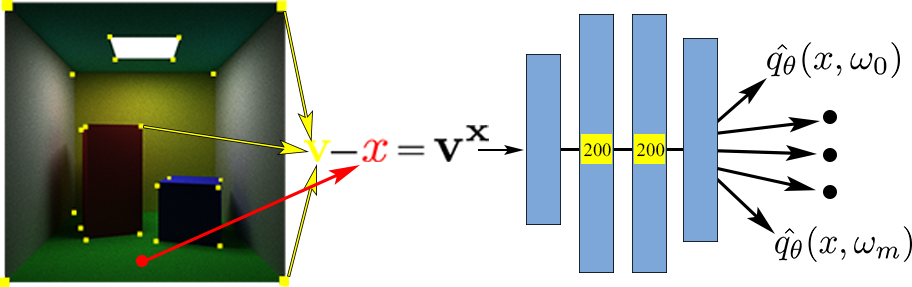
\includegraphics[width=0.9\textwidth]{images/fwd_pass_process.png}   
\caption{An illustration of the process for a forward pass on the ANN used for the Neural-Q path tracer. Starting with the scene on the left, all vertices in the scene are converted into a coordinate system relative to the point $x$, producing $\mathbf{v^x}$. This is passed to the input layer of the ANN which then computes a forward pass through the two hidden layers fully connected layers, each with a width of $200$ neurons to the output layer. The output layers width is equal to the number of discrete incident directions $m$ used in the approximation of the incident radiance function. Each output represents the approximated incident radiance on the position $x$ for every discrete incident direction $\hat{q_\theta}(x, \omega_k)$ $\forall k = 1, ..., m$.}
\label{fig:nn_radiance_estimate_illustration}
\end{figure}

As shown in the illustration in Figure \ref{fig:nn_radiance_estimate_illustration}, the ANN consists of an input layer consisting of $z$ neurons, where $z$ is the the total number of vertices in the scene. The input is then all vertices in the scene converted into a coordinate system around the intersection position $x$, $\mathbf{v^x}$. Then there are 2 hidden fully connected layers, where each hidden layer is followed by a rectifier of non-linearity activation function (ReLU) \cite{nair2010rectified}. The output layer consists of a neuron to output the approximated incident radiance from every direction of the discretized hemisphere around the intersection point $x$. The choice to use only two fully connected hidden layers was made to reduce time spent on computing forward passes and training the network during the rendering of an image. Whilst still having two hidden layers allows the ANN to represent an arbitrary decision boundary for approximating incident radiance at any given position which is a 5D function $L_i(x, \omega)$, where $x \in \mathbb{R}^3$  and $\omega \in \mathbb{R}^2$. However, for scenes with more complex geometry than those experimented on may require more hidden layers and/or neurons in hidden layers in order to accurately approximate $L_i(x, \omega)$ \cite{ren2013global}.\\

Training the ANN is where the main difference arises compared to the supervised learning case. Recall from section \ref{sec:bootstrapping}, in the reinforcement learning case there is no large training data set available for learning the optimal value function directly. Hence, bootstrapping is used in TD-learning methods in order to learn online by continually updating the estimate of the optimal value function as data is received. This is otherwise known as learning from experience \cite{sutton2011reinforcement}. The loss function in Equation \ref{eq:neural_q_loss} does exactly that, where the loss is described in terms of some immediate reward which is the emitted radiance $L_e$ term, and partially on the current estimate of radiance incident from direction $\omega$:

$$\text{TD Error: } \triangle \hat{q_\theta}(x, \omega) = \left( L_e(y, -\omega) + \left[ \max_{\omega_i} \left(\hat{q_\theta}(y, \omega_i) f_s(\omega_i, y, \omega) (\omega_i \cdot \mathbf{n}) \right) \right] \right) - \hat{q_\theta}(x, \omega)$$

So, to compute this loss an initial forward pass on the network must be made to determine the value of $\hat{q_\theta}(x, \omega)$, then a second pass must be made to calculate $max_{\omega_i} \hat{q_\theta}(y, \omega_i)$. All other terms are a result of experience and are calculated in the path tracing algorithm. After the loss is calculated backpropagation is used to compute the partial derivative of the loss with w.r.t to each parameter. Then another pass can be made through the network to update the networks weights using the partial derivatives calculated in the previous step with an optimizer, in this case I use the Adam optimizer. While there is no guarantee, in practice ver many iterations of this learning procedure, the ANNs estimate of incident radiance for a discrete set of directions $\omega_k$ for any point $x$ in the scene should move towards a local optimum \cite{deep_rl_function_approx}.

\subsection{Neural-Q Path Tracing Algorithm}

With an ANN and a method for training it to learn the the incident radiance from $n$ discrete directions on a point detailed, a modified Monte Carlo path tracing algorithm which uses this ANNs predictions for importance sampling directions to continue light paths must be introduced. Algorithm \ref{alg:neural_q_pathtracer} renders a single image using $N$ sampled light paths per pixel to compute the colour estimate of each pixel by Monte Carlo path tracing. Similarly to the Expected Sarsa path tracer detailed in Algorithm \ref{alg:expected_sarsa_pathtracer}, the Neural-Q path tracer estimates the radiance distribution at the intersection point of a light path and samples a direction to continue the light path in proportional to this distribution. This radiance distribution is also used as the probability density function in the Monte Carlo estimate of the rendering equation \ref{eq:rendering_eq_monte_carlo} to reduce the variance in the approximation of the outgoing radiance $L_o$, leading to a reduction in image noise. The algorithm also trains online, meaning it progressively reduces noise in the image as simulates more light paths. Once again the $\rho_i$ term is the probability density function over the hemisphere of directions $\Omega$ at intersection point $x$ to continue a light path in, evaluated for the sampled direction $\omega_i$. This can be calculated using Equation \ref{eq:mc_expected_sarsa_pdf} in section \ref{sec:expected_sarsa_path_tracer}. There are four additions to this algorithm compared to the default forward path tracing algorithm \ref{alg:forward_path_tracing}:

\subsubsection*{Addition 1: Minibatching}
In order to yield smoother sample gradient for training, a minibatching method is used where the gradient information for light paths is accumulated over a batch to train the network with. This was proven to be succesful for a range of physical control tasks in\cite{lillicrap2015continuous}. While Algorithm \ref{alg:neural_q_pathtracer} iterates through the batches to clearly represent the steps the algorithm takes, in practice all computation with the batch loops are done in parallel. 

\subsubsection*{Addition 2: Sample direction using decaying $\epsilon$-\textit{greedy} policy}
The Neural-Q path tracer follows a decaying $\epsilon$-\textit{greedy} policy to either sample a ray direction proportional to the estimated radiance distribution at the intersection position. Or, randomly sample one of the discrete directions in the discretized hemisphere centred at the intersection point. This choice is made depending on the value of $\epsilon$. Where $\epsilon \in [0,1]$, a random number $r \in [0,1]$ is sampled. If $r > \epsilon$ then the so called \textit{greedy} strategy is chosen. This is where a direction is sampled proportional to the radiance distribution formed by normalizing the Q-values produced by a forward pass on the network using $\mathbf{v^x}$ as input, where $x$ is the current intersection position of the light path. Otherwise, a random direction $\omega_k$ is selected from the discrete set directions $\omega_k$ for $i = 1,...,n$ for the adaptive quadrature at the point of intersection. 

\subsubsection*{Addition 3: Training the ANN}
This modification trains the ANN to improve its approximation of the incident radiance at any point $x$ in the scene for the set of discrete angle $\omega_k$ in the adaptive quadrature centred at $x$. To do so, the algorithm computes the loss function in \ref{eq:neural_q_loss}, by running a forward pass on the ANN to get the approximated incident radiance in the discrete directions $\omega_k$ $\forall k=1,...,n$ for both the position $x$, as well as the next intersected position $y$. The loss is then used to train the network using the process described in section \ref{sec:ann_architecture}. The policy followed for selecting a direction to continue a light path in is different to that of selecting a direction Q-value for training with in $\hat{q_theta}(y, \omega)$ for bootstrapping. This is instead chosen according to the direction with the highest incident radiance from $y$ as shown in \ref{eq:neural_q_loss}. This is the reason why deep-Q learning is an off-policy algorithm.\\ 

Whilst a replay buffer was not used in the Neural-Q path tracer, what it hopes to achieve is partially covered by the Neural-Q path tracing algorithm. A replay buffer was originally introduced for deep Q-learning in \cite{mnih2013playing} for training an AI agent to play a variety of Atari games by learning a good approximation of the optimal value function using deep Q-learning. Where the replay buffer stores transitions between from state-action pairs and the corresponding reward received $e_t = (S_t, A_t, R_t, S_{t+1})$. The replay buffer is then sampled from to make up part of the minibatch to train the network with. This is known as experience replay and is used to avoid giving the network highly correlated data to train on as a result of learning online, taking one action  in a particular states may affect the probability of selecting another action in the next state. Neural networks make the assumption that the training data is independently and identically distributed (i.i.d), which was not the case for consecutive states in Atari games. Therefore, by sampling from a replay buffer the variance in consecutive weight updates is reduced as they updates are no longer highly correlated with one another compared to using standard Q-learning \cite{sutton2011reinforcement}. Rather then storing transitions in a buffer to make up a minibatch for training, a batch of rays are continually traced and trained together. This avoids strong correlations between training iterations, reducing the variance in consecutive weight updates. However, it is likely there still is some correlation in the initial consecutive training iterations for light paths sampled from spatially local pixel positions in the image plane, so using some form of replay buffer like that suggested in \cite{muller2018neural} may further reduce the variance in consecutive weight updates.

\subsubsection*{Addition 4: Decaying decaying $\epsilon$-\textit{greedy}}
As part of the decaying $\epsilon$-\textit{greedy} policy, the value of $\epsilon$ is decreased after $1$ sampled light path is computed through every pixel in the image. Meaning, according to Algorithm \ref{alg:neural_q_pathtracer}, this represents a single epoch. This is a reasonable point to decay epsilon as for an average light path length of $30$ for each sampled pixel in a $512x512$ image with a minibatch size of $1024$, approximately $7,680$ training updates are made on the network. As discussed in section \ref{eq:exploration_vs_exploitation}, the decaying $\epsilon$-\textit{greedy} policy means the makes sure the path tracer at first prioritises exploration of which direction contribute the most radiance. As training progresses, the path tracers policy alters more towards exploiting by sampling directions to continue light paths in based on the current estimated radiance distribution at their intersections points. This behaviour is desirable, as by focusing on exploitation to early, the path tracer may not sample seemingly unfavourable directions in the short term which after more reflections off surfaces lead to a large amount of incident radiance to the point.

\begin{algorithm}[H]
\label{alg:neural_q_pathtracer}
\SetKwProg{Fn}{Function}{ }{end}
\SetAlgoLined
 \Fn{renderImage(camera, scene, decay, $\epsilon$)}{  
   $ANN = \text{loadANN()}$\\
   \For{$i = 1$ \KwTo $N$}{
       \tcc{Addition (1)}
       \For{$b = 1$ \KwTo $\text{Batches}$}{
           \For{$k = 1$ \KwTo $\text{BatchSize}$}{
               $p \leftarrow \text{getPixel(b,k)}$\\
               $ray \leftarrow \text{initializeRay}(p, camera)$\\
               \For{$j=1$ \KwTo $\infty$}{
                   $(y, \mathbf{n}, L_e) \leftarrow \text{closestIntersection}(ray, scene)$\\
                   \If{$j > 1$}{
                       \tcc{Addition (2)}
                       $(\omega_i, \rho_i, f_s) \leftarrow \text{sampleRayDirEpsilonGreedy}(\epsilon, y)$\\
                       \tcc{Addition (3)}
                       $\hat{q_\theta}x \leftarrow ANN.getQValue(ray.x, ray.\omega, scene)$\\
                       $\hat{q_\theta}y \leftarrow ANN.getMaxQValue(y, scene)$\\
                       $\triangle \hat{q}_\theta x \leftarrow L_e +  \left(\hat{q_\theta}y  \cdot f_s \cdot (\omega_i \cdot \mathbf{n}) \right) - \hat{q_\theta}x$\\
                       $ANN.\text{train}(\triangle \hat{q}_\theta x)$
                   }
                   \If{$\text{noIntersection}(y) \ \Or \ \text{areaLightIntersection}(y)$}{
                       $ray.throughput \leftarrow ray.throughput \cdot L_e$\\
                       $\text{updatePixelColourEstimate}(p, ray.throughput)$\\
                       $\Break$
                   }
                  $ray.throughput \leftarrow ray.throughtput \cdot f_s \cdot (\omega_i \cdot \mathbf{n}) / \rho_i$\\
                  $ray \leftarrow (y, \omega_i)$
               }
           }
       }
       \tcc{Addition (4)}
       $\epsilon \leftarrow \epsilon - decay$
   }
 }
 \caption{Neural-Q forward path tracer. Given a camera position, scene geometry, epsilon and epsilon decay, this algorithm will render a single image using deep Q-learning loss to progressively reduce image noise. Where $N$ is the pre-specified number of sampled light paths per pixel.}
\end{algorithm}


\begin{comment}
% Advantages
% Less memory
% Same architecture can be applied to scene rather then applying complex data structures to the scene

Deep Learning for denoising light transport simulation rendering methods:
\begin{itemize}
\item \cite{zheng2018learning} - Uses a DNN to pre-train on a scene to figure out which pixels require more samples rather then just uniformly sampling the same amount of light rays for every pixel.

\item \cite{muller2018neural} - Uses a DNN for both online learning in light path construction and also introduces i for Primary Sample Space importance sampling. Performs well, not usable currently due to bottleneck of inference

"At any given point during rendering, a sample is generated by drawing a random pair u ∈ [0, 1] passing it through the inverted coupling layers in reverse order, and transforming to the range of cylindrical coordinates to obtain ω." - This means it simply gives a direction rather then return the value of directions around it, does this mean there is no stochasticity when sampling a new direction? Everytime we intersect with a world coordinate we will sample a ray in the same direction if no training occurs? Dont make this claim just allude to importance sampling over directions is better

\item \cite{keller2019integral} - Introduces a range of methods for NN, most related to mine is using NN to output Q-value of the light source. Neural network determines which light source to compute direct illumination from for a given normal, intersection point and incoming direction to the intersection point. They also use it to determine visibility, which light sources contribute the most to a point, as well as a direct approximation of radiance
\end{itemize}


{\bf A topic-specific chapter, of roughly $15$ pages} 
\vspace{1cm} 

\noindent
This chapter is intended to describe what you did: the goal is to explain
the main activity or activities, of any type, which constituted your work 
during the project.  The content is highly topic-specific, but for many 
projects it will make sense to split the chapter into two sections: one 
will discuss the design of something (e.g., some hardware or software, or 
an algorithm, or experiment), including any rationale or decisions made, 
and the other will discuss how this design was realised via some form of 
implementation.  

This is, of course, far from ideal for {\em many} project topics.  Some
situations which clearly require a different approach include:

\begin{itemize}
\item In a project where asymptotic analysis of some algorithm is the goal,
      there is no real ``design and implementation'' in a traditional sense
      even though the activity of analysis is clearly within the remit of
      this chapter.
\item In a project where analysis of some results is as major, or a more
      major goal than the implementation that produced them, it might be
      sensible to merge this chapter with the next one: the main activity 
      is such that discussion of the results cannot be viewed separately.
\end{itemize}

\noindent
Note that it is common to include evidence of ``best practice'' project 
management (e.g., use of version control, choice of programming language 
and so on).  Rather than simply a rote list, make sure any such content 
is useful and/or informative in some way: for example, if there was a 
decision to be made then explain the trade-offs and implications 
involved.

\section{Example Section}

This is an example section; 
the following content is auto-generated dummy text.
\lipsum

\subsection{Example Sub-section}

\begin{figure}[t]
\centering
foo
\caption{This is an example figure.}
\label{fig}
\end{figure}

\begin{table}[t]
\centering
\begin{tabular}{|cc|c|}
\hline
foo      & bar      & baz      \\
\hline
$0     $ & $0     $ & $0     $ \\
$1     $ & $1     $ & $1     $ \\
$\vdots$ & $\vdots$ & $\vdots$ \\
$9     $ & $9     $ & $9     $ \\
\hline
\end{tabular}
\caption{This is an example table.}
\label{tab}
\end{table}

\begin{algorithm}[t]
\For{$i=0$ {\bf upto} $n$}{
  $t_i \leftarrow 0$\;
}
\caption{This is an example algorithm.}
\label{alg}
\end{algorithm}

\begin{lstlisting}[float={t},caption={This is an example listing.},label={lst},language=C]
for( i = 0; i < n; i++ ) {
  t[ i ] = 0;
}
\end{lstlisting}

This is an example sub-section;
the following content is auto-generated dummy text.
Notice the examples in Figure~\ref{fig}, Table~\ref{tab}, Algorithm~\ref{alg}
and Listing~\ref{lst}.
\lipsum

\subsubsection{Example Sub-sub-section}

This is an example sub-sub-section;
the following content is auto-generated dummy text.
\lipsum

\paragraph{Example paragraph.}

This is an example paragraph; note the trailing full-stop in the title,
which is intended to ensure it does not run into the text.


\subsection{Plan}

% I imagine this section to be like a mini paper starting at new method

\textbf{Breakdown}
\begin{enumerate}

\item State learning rule for deep Q-learning and the difference from deep Q-learning to q-learning. Maybe some of the difficulties associated with deep q-learning versus q-learning, and some of the general advantages. 

\item Derive the learning rule for deep q-learning network which I used, once again justifying terms throughout the derivation.

\item Explain concept of eta-greedy policy used. Explain exploration vs exploitation but we will talk about this more later

\item Describe how the current method is used for diffuse surfaces. Introduce the pseudo code for the new algorithm. Give a description of each stage and what it does. Relating back to properties such as bias rendering and pointing out assumption made by the path tracer.

\item Present and explain the network architecture. Explain in depth about how the state was modelled as a point relative to all vertices to give the network information about the position of the vertex relative to the rest of the world compared to passing in a single position. Relate this to Atari games, we get an image showing where we are relative to the world rather than just a single position in the world.

\item Present some results side by side against a default path tracer and Nvidia's reinforcement learning approach. Pointing out aspects of the image and reasoning for certain parts.

\end{enumerate}
\end{comment}

\end{document}